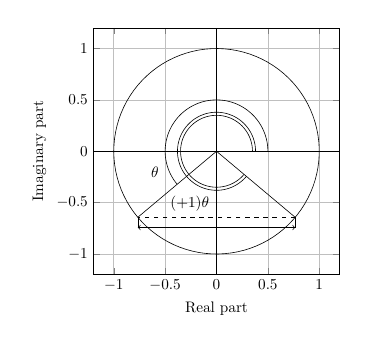
\begin{tikzpicture}[scale=.55]
	\begin{axis}[grid=both,
		xlabel = Real part,
		ylabel = Imaginary part,
		%		axis equal,
		axis equal image,
		ymin = -1.2,
		ymax = 1.2,
		xmin = -1.2,
		xmax = 1.2]
		\addplot [domain=-180:180, samples=100] ({cos(x)},{sin(x)});
		\draw (-1.2,0) -- (1.2,0);
		\draw (0,-1.2) -- (0,1.2);
		\draw (0,0) -- ({cos(40)},{-sin(40)});
		\draw (0,0) -- ({-cos(40)},{-sin(40)});
		\addplot [domain=0:220, samples=100] ({.5*cos(x)},{.5*sin(x)});
		\node at (-.6,-.2) {$ \delayn \theta $};
		\addplot [domain=0:320, samples=100] ({.38*cos(x)},{.38*sin(x)});		
		\addplot [domain=0:320, samples=100] ({.35*cos(x)},{.35*sin(x)});	
		\node at (-.26,-.51) {$ (\delayn+1) \theta $};	
		\draw[dashed] ({cos(40)},{-sin(40)}) -- ({-cos(40)},{-sin(40)});
		\draw[<->] ({cos(40)},{-sin(40)-.1}) -- ({-cos(40)},{-sin(40)-.1});
		\draw ({cos(40)},{-sin(40)-.1}) -- ({cos(40)},{-sin(40)});
		\draw (-{cos(40)},{-sin(40)-.1}) -- (-{cos(40)},{-sin(40)});
		\node at (0.05,{-sin(40)-.22}) {$ \gpos $};
	\end{axis}
\end{tikzpicture}